\section{Graph Approximations}
\begin{frame}{What is a fractal?}
    You know it, when you see it!

    \begin{columns}[c]
        \column{0.33\textwidth}
        \begin{figure}
            \centering
            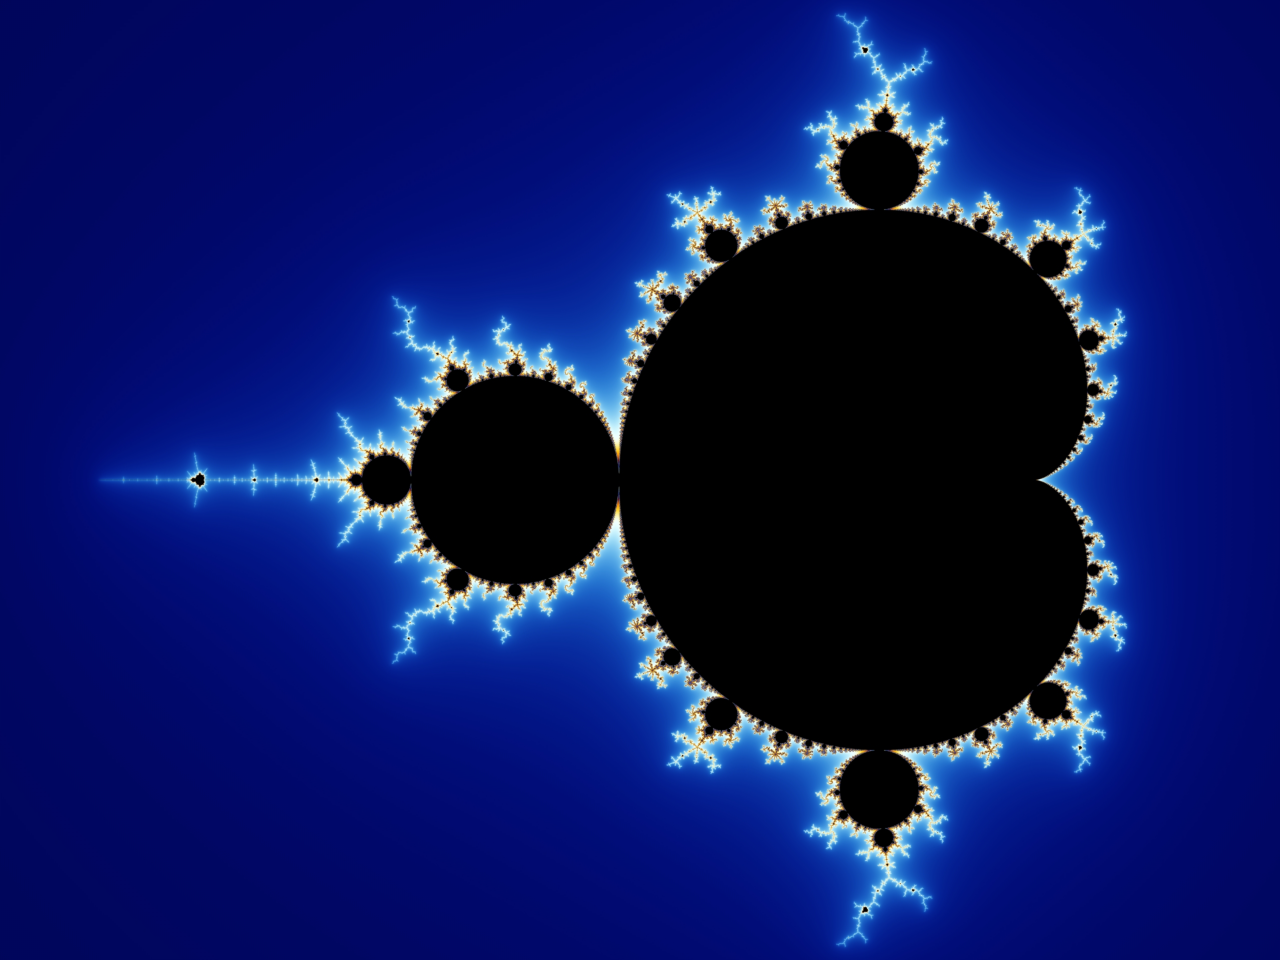
\includegraphics[height=5em]{images/mandelbrot.pdf}
            \caption{Mandelbrot set}
        \end{figure}
        \column{0.33\textwidth}
        \begin{figure}
            \centering
            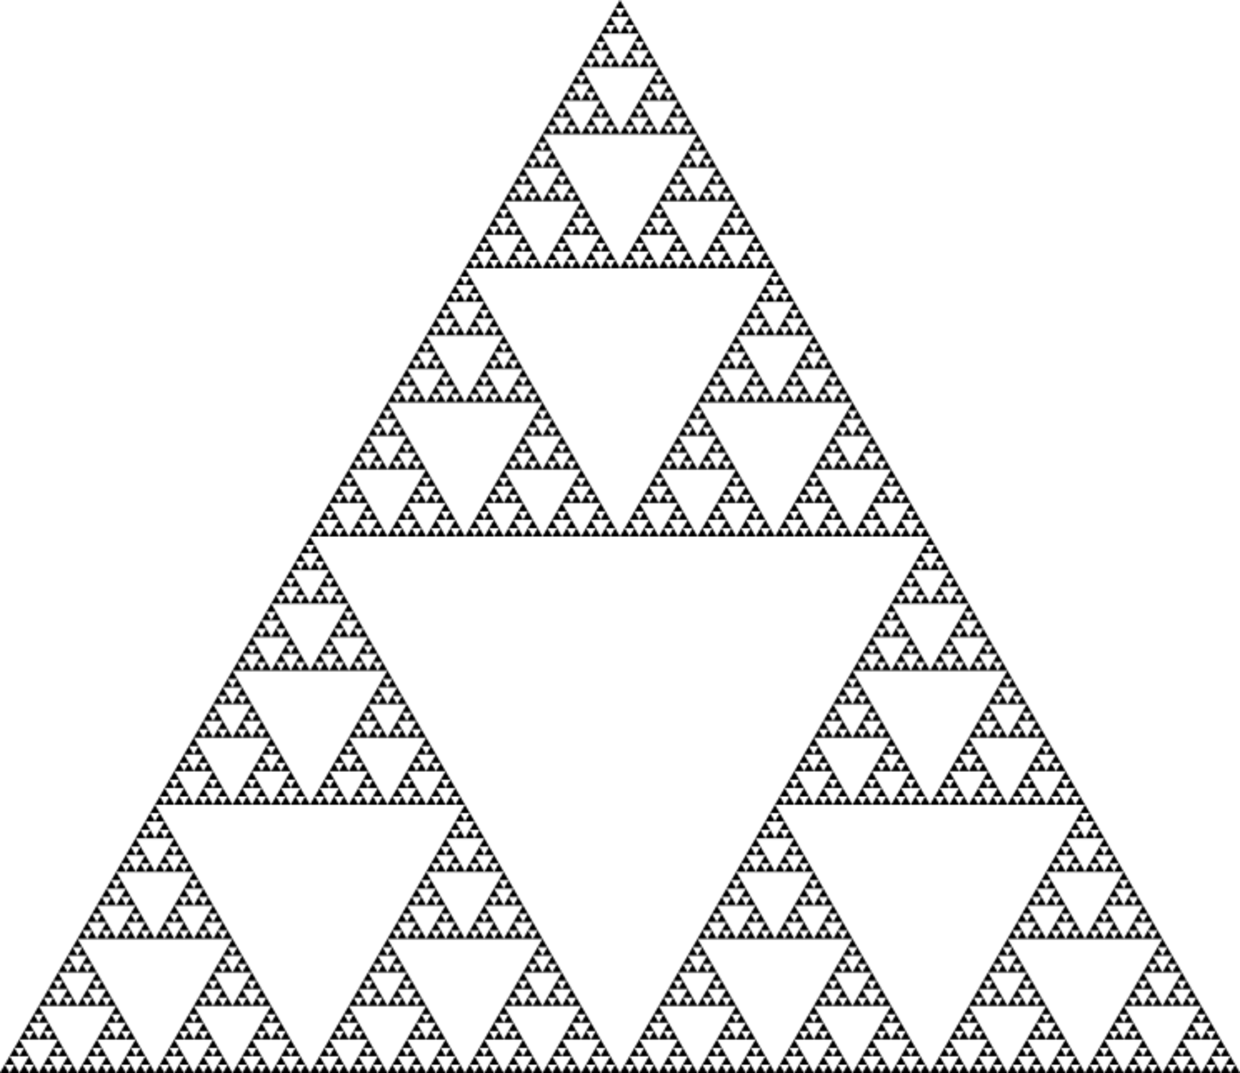
\includegraphics[height=5em]{images/sierpinksi.pdf}
            \caption{Sierpinksi gasket}
        \end{figure}
        \column{0.33\textwidth}
        \begin{figure}
            \centering
            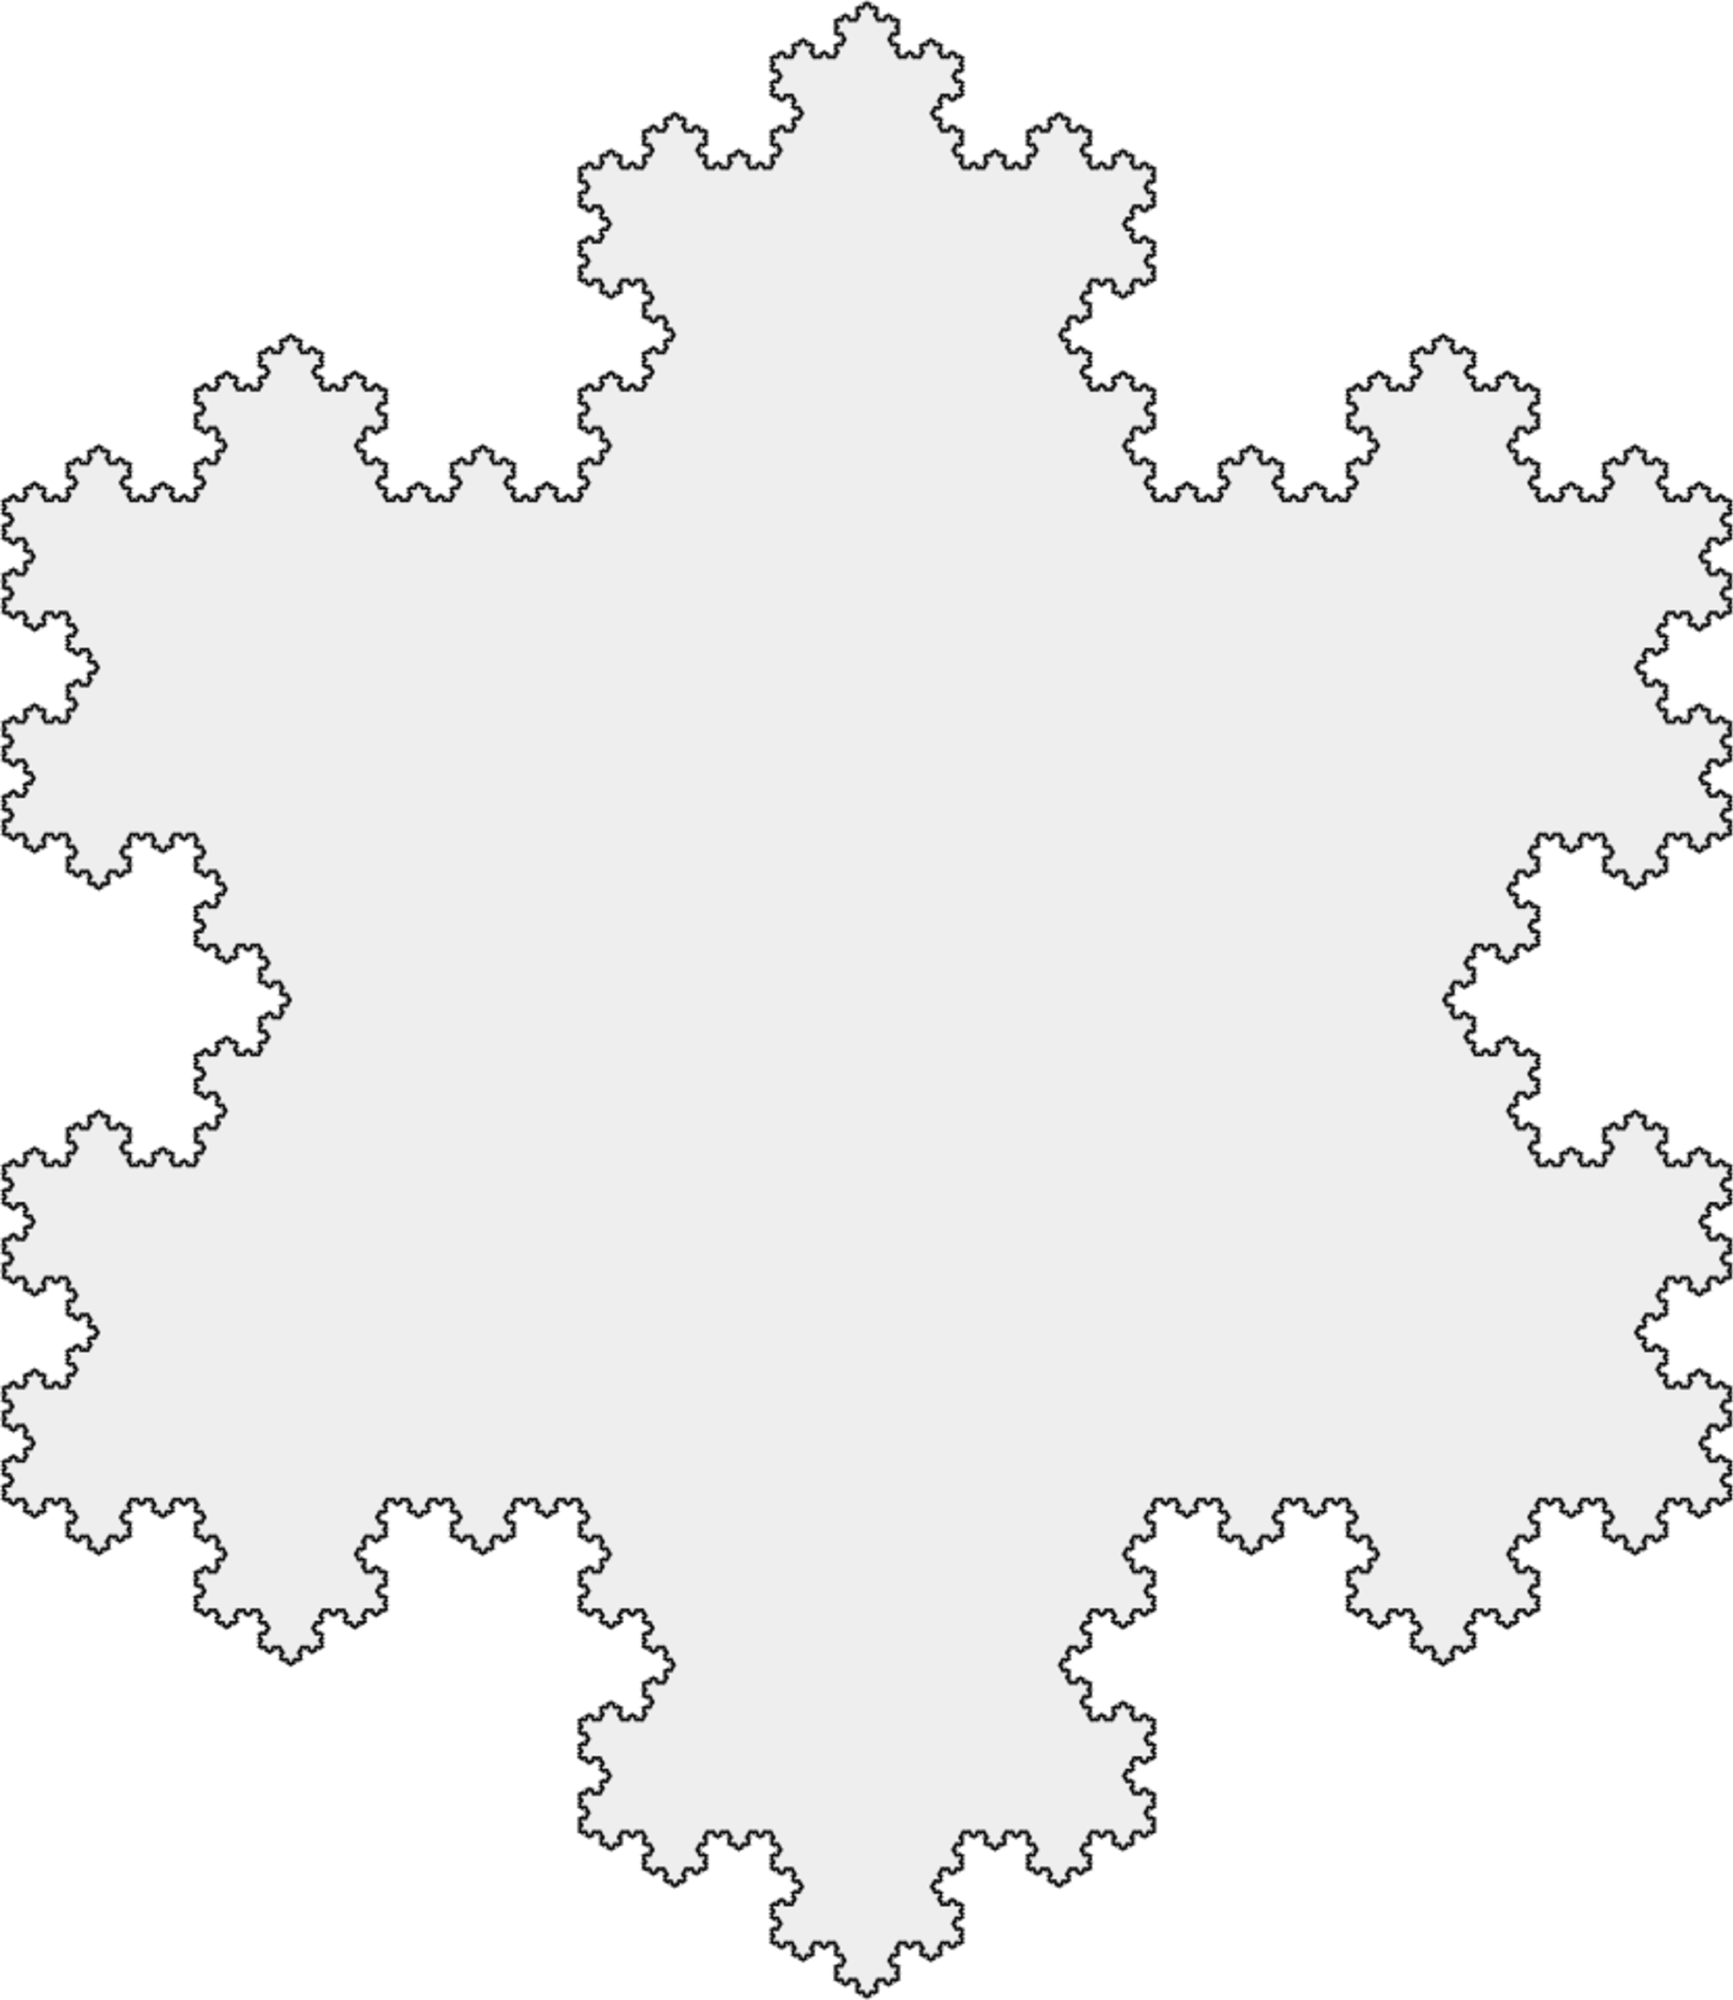
\includegraphics[height=5em]{images/snowflake.pdf}
            \caption{Koch snowflake}
        \end{figure}
    \end{columns}

    Common features: 
    \begin{itemize}
        \item self-similarity
        \item roughness
        \item infinitely detailed
        \item generate complex structure from very simple procedure (e.g. from iterated function systems)
    \end{itemize}
\end{frame}

\begin{frame}{Iterated function systems}
    \begin{definition}
        An \textit{iterated function system (IFS)} is a family \(F = \{ F_i: \R^d \to \R^d : 1 \leq i \leq N \ \} \) of contractions.
    \end{definition}

    \begin{theorem}[Hutchinson, 1981]
        There is a unique non-empty, compact set \(K \subset \R^d \) so that
        \[ K = F(K) := \bigcup_i F_i(K). \]
    \end{theorem}

    \begin{example}
        \begin{columns}[c]
            \column{0.7\textwidth}
            (a) \textbf{Sierpinksi gasket:} Let \(V_0 := \{\textcolor{red}{q_0}, \textcolor{green}{q_1}, \textcolor{blue}{q_2} \} \) be the verticies of a proper triangle. Then these contractions characterize the Sierpinksi gasket \(SG \subset \R^2 \):
            \[ F_i(x) := \frac{1}{2}(x - q_i) + q_i \]
            \column{0.3\textwidth}
            \begin{figure}
                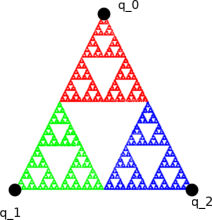
\includegraphics[height=7em]{images/colored.pdf}
            \end{figure}
        \end{columns}
    \end{example}
\end{frame}

\begin{frame}{Addressing points in IFS fractals}
    \addtocounter{definition}{-1}
    \begin{example}[Cont.]
        (b) \textbf{Unit interval (not a fractal but self-similar):} Choose \(V_0 := \{q_0 = 0, q_1 = 1 \} \). Then
        \[ F_i(x) := \frac{1}{2}(x - q_i) + q_i \]
        gives us the unit interval \(I \subset \R \).
    \end{example}

    Iteratively, define \(V_m := \bigcup_i F_i(V_{m-1}) \) and note that one can write
    \[ V_m = \bigcup_{| \omega | = m} F_\omega(V_0), \quad \text{where } F_\omega := F_{\omega_1} \circ \cdots \circ F_{\omega_m} \]
    and \(\omega \in \{1, \dots, N \}^m \) is a \textit{word} of length \(| \omega | = m \).

    So, \(V_m \subset V_{m+1} \) and every point \(x \in V_* := \bigcup_{m \geq 0} V_m \) can be written as \(x = F_\omega q_i \).  Every \(x \in V_m \setminus V_0 \) has exactly two addresses since \(F_0 q_1 = F_1 q_0 \), \(F_1 q_2 = F_2 q_1 \) and \(F_2 q_0 = F_0 q_2 \).
    Finally: Convince yourself, that \(K = \overline{V_*} \).
\end{frame}

\begin{frame}{Graph approximations}
    \begin{example}[Graph approximations]
        \begin{enumerate}
            \item Unit interval:
        \begin{columns}[c]
            \column{0.33\textwidth}
            \begin{figure}
                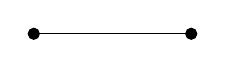
\begin{tikzpicture}[scale=2]
                    \draw (0,0) -- (1,0);
                    \filldraw [black] (0,0) circle (1pt);
                    \filldraw [black] (1,0) circle (1pt);
                \end{tikzpicture}\\
                \centering
                \(\Gamma_0 \)
            \end{figure}
            \column{0.33\textwidth}
            \begin{figure}
                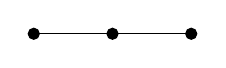
\begin{tikzpicture}[scale=2]
                    \draw (0,0) -- (1,0);
                    \filldraw [black] (0,0) circle (1pt);
                    \filldraw [black] (1,0) circle (1pt);
                    \filldraw [black] (0.5,0) circle (1pt);
                \end{tikzpicture}\\
                \centering
                \(\Gamma_1 \)
            \end{figure}
            \column{0.33\textwidth}
            \begin{figure}
                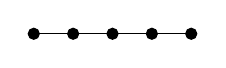
\begin{tikzpicture}[scale=2]
                    \draw (0,0) -- (1,0);
                    \filldraw [black] (0,0) circle (1pt);
                    \filldraw [black] (1,0) circle (1pt);
                    \filldraw [black] (0.5,0) circle (1pt);
                    \filldraw [black] (0.25,0) circle (1pt);
                    \filldraw [black] (0.75,0) circle (1pt);
                \end{tikzpicture}\\
                \centering
                \(\Gamma_2 \)
            \end{figure}
        \end{columns}
        \item Sierpinksi gasket:
        \begin{columns}[c]
            \column{0.33\textwidth}
            \begin{figure}
                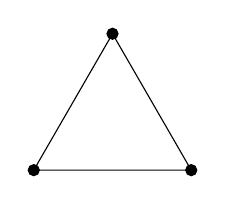
\begin{tikzpicture}[scale=2]
                    \draw (0,0) -- (1,0) -- (0.5,0.866) -- (0,0);
                    \filldraw [black] (0,0) circle (1pt);
                    \filldraw [black] (1,0) circle (1pt);
                    \filldraw [black] (0.5,0.866) circle (1pt);
                \end{tikzpicture}\\
                \centering
                \(\Gamma_0 \)
            \end{figure}
            \column{0.33\textwidth}
            \begin{figure}
                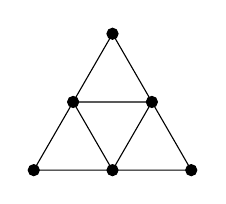
\begin{tikzpicture}[scale=2]
                    \draw (0,0) -- (1,0) -- (0.5,0.866) -- (0,0);
                    \draw (0.5,0) -- (0.25,0.433) -- (0.75,0.433) -- (0.5,0);
                    \filldraw [black] (0,0) circle (1pt);
                    \filldraw [black] (1,0) circle (1pt);
                    \filldraw [black] (0.5,0.866) circle (1pt);
                    \filldraw [black] (0.5,0) circle (1pt);
                    \filldraw [black] (0.25,0.433) circle (1pt);
                    \filldraw [black] (0.75,0.433) circle (1pt);
                \end{tikzpicture}\\
                \centering
                \(\Gamma_1 \)
            \end{figure}
            \column{0.33\textwidth}
            \begin{figure}
                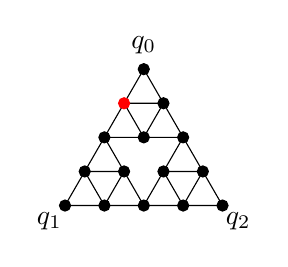
\begin{tikzpicture}[scale=2]
                    \draw (0,0) -- (1,0) -- (0.5,0.866) -- (0,0);
                    \draw (0.5,0) -- (0.25,0.433) -- (0.75,0.433) -- (0.5,0);
                    \draw (0.5,0.433) -- (0.375,0.6495) -- (0.625,0.6495) -- (0.5,0.433);
                    \draw (0.25,0) -- (0.125,0.2165) -- (0.375,0.2165) -- (0.25,0);
                    \draw (0.75,0) -- (0.625,0.2165) -- (0.875,0.2165) -- (0.75,0);
                    \filldraw [black] (0,0) circle (1pt);
                    \node[yshift=-2mm, xshift=-2mm] at (0,0) {\(q_1\)};
                    \filldraw [black] (1,0) circle (1pt);
                    \node[yshift=-2mm, xshift=2mm] at (1,0) {\(q_2\)};
                    \filldraw [black] (0.5,0.866) circle (1pt);
                    \node[yshift=3mm, xshift=0mm] at (0.5,0.866) {\(q_0\)};
                    \filldraw [black] (0.5,0) circle (1pt);
                    \filldraw [black] (0.25,0.433) circle (1pt);
                    \filldraw [black] (0.75,0.433) circle (1pt);
                    \filldraw [black] (0.25,0) circle (1pt);
                    \filldraw [black] (0.75,0) circle (1pt);
                    \filldraw [black] (0.125,0.2165) circle (1pt);
                    \filldraw [black] (0.375,0.2165) circle (1pt);
                    \filldraw [black] (0.625,0.2165) circle (1pt);
                    \filldraw [black] (0.875,0.2165) circle (1pt);
                    \filldraw [black] (0.5, 0.433) circle (1pt);
                    \filldraw [red] (0.375,0.6495) circle (1pt);
                    \filldraw [black] (0.625,0.6495) circle (1pt);
                \end{tikzpicture}\\
                \centering
                \(\Gamma_2 \)
            \end{figure}
        \end{columns}
    \end{enumerate}
    \end{example}
    The red vertex is in \(V_2 \setminus V_1 \) and is addressed via \(x = F_{(0, 1)}q_0 = F_{(0,0)}q_1 \).
\end{frame}

\begin{frame}{Finite ramification and graph approximations}
    \begin{definition}
        \begin{enumerate}
            \item If \(\omega \) is a word of with length \(| \omega | = m \), we call \(F_\omega (K) \) a \textit{cell} of level \(m \).
            \item If two distinct cells of level \(m \) intersect in at most finitely many points, we say that \(K \) is \textit{finitely ramified}.
        \end{enumerate}
    \end{definition}

    In the case of \(K \in \{I, SG \} \), two distinct \(m \) level cells intersect in at most one point and the set of those \textit{junction points} is \(V_m \setminus V_0 \). We can thus define a relation on the set \(V_m \) through
    \[ x \sim_m y :\Leftrightarrow \text{there is a } \omega \text{ of length } | \omega | = m \text{ so that } x, y \in F_\omega K. \]

    Now, we can consider graphs \(\Gamma_m := (V_m, \sim_m) \).
\end{frame}

\begin{frame}{Graph approximations}
    \begin{example}[Graph approximations]
        \begin{enumerate}
            \item Unit interval:
        \begin{columns}[c]
            \column{0.33\textwidth}
            \begin{figure}
                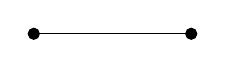
\begin{tikzpicture}[scale=2]
                    \draw (0,0) -- (1,0);
                    \filldraw [black] (0,0) circle (1pt);
                    \filldraw [black] (1,0) circle (1pt);
                \end{tikzpicture}\\
                \centering
                \(\Gamma_0 \)
            \end{figure}
            \column{0.33\textwidth}
            \begin{figure}
                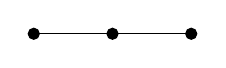
\begin{tikzpicture}[scale=2]
                    \draw (0,0) -- (1,0);
                    \filldraw [black] (0,0) circle (1pt);
                    \filldraw [black] (1,0) circle (1pt);
                    \filldraw [black] (0.5,0) circle (1pt);
                \end{tikzpicture}\\
                \centering
                \(\Gamma_1 \)
            \end{figure}
            \column{0.33\textwidth}
            \begin{figure}
                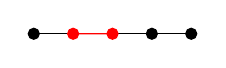
\begin{tikzpicture}[scale=2]
                    \draw (0,0) -- (1,0);
                    \filldraw [black] (0,0) circle (1pt);
                    \filldraw [black] (1,0) circle (1pt);
                    \filldraw [red] (0.25,0) -- (0.5,0) circle (1pt);
                    \filldraw [red] (0.25,0) circle (1pt);
                    \filldraw [red] (0.25,0) -- (0.5,0);
                    \filldraw [black] (0.75,0) circle (1pt);
                    %\draw[line width=2mm,red](0.25,0) -- (0.5,0);
                \end{tikzpicture}\\
                \centering
                \(\Gamma_2 \)
            \end{figure}
        \end{columns}
        \item Sierpinksi gasket:
        \begin{columns}[c]
            \column{0.33\textwidth}
            \begin{figure}
                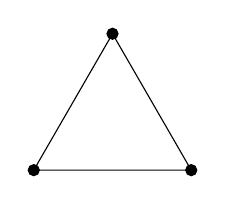
\begin{tikzpicture}[scale=2]
                    \draw (0,0) -- (1,0) -- (0.5,0.866) -- (0,0);
                    \filldraw [black] (0,0) circle (1pt);
                    \filldraw [black] (1,0) circle (1pt);
                    \filldraw [black] (0.5,0.866) circle (1pt);
                \end{tikzpicture}\\
                \centering
                \(\Gamma_0 \)
            \end{figure}
            \column{0.33\textwidth}
            \begin{figure}
                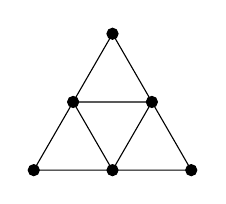
\begin{tikzpicture}[scale=2]
                    \draw (0,0) -- (1,0) -- (0.5,0.866) -- (0,0);
                    \draw (0.5,0) -- (0.25,0.433) -- (0.75,0.433) -- (0.5,0);
                    \filldraw [black] (0,0) circle (1pt);
                    \filldraw [black] (1,0) circle (1pt);
                    \filldraw [black] (0.5,0.866) circle (1pt);
                    \filldraw [black] (0.5,0) circle (1pt);
                    \filldraw [black] (0.25,0.433) circle (1pt);
                    \filldraw [black] (0.75,0.433) circle (1pt);
                \end{tikzpicture}\\
                \centering
                \(\Gamma_1 \)
            \end{figure}
            \column{0.33\textwidth}
            \begin{figure}
                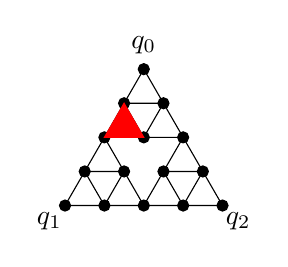
\begin{tikzpicture}[scale=2]
                    \draw (0,0) -- (1,0) -- (0.5,0.866) -- (0,0);
                    \draw (0.5,0) -- (0.25,0.433) -- (0.75,0.433) -- (0.5,0);
                    \draw (0.5,0.433) -- (0.375,0.6495) -- (0.625,0.6495) -- (0.5,0.433);
                    \draw (0.25,0) -- (0.125,0.2165) -- (0.375,0.2165) -- (0.25,0);
                    \draw (0.75,0) -- (0.625,0.2165) -- (0.875,0.2165) -- (0.75,0);
                    \filldraw [black] (0,0) circle (1pt);
                    \node[yshift=-2mm, xshift=-2mm] at (0,0) {\(q_1\)};
                    \filldraw [black] (1,0) circle (1pt);
                    \node[yshift=-2mm, xshift=2mm] at (1,0) {\(q_2\)};
                    \filldraw [black] (0.5,0.866) circle (1pt);
                    \node[yshift=3mm, xshift=0mm] at (0.5,0.866) {\(q_0\)};
                    \filldraw [black] (0.5,0) circle (1pt);
                    \filldraw [black] (0.25,0.433) circle (1pt);
                    \filldraw [black] (0.75,0.433) circle (1pt);
                    \filldraw [black] (0.25,0) circle (1pt);
                    \filldraw [black] (0.75,0) circle (1pt);
                    \filldraw [black] (0.125,0.2165) circle (1pt);
                    \filldraw [black] (0.375,0.2165) circle (1pt);
                    \filldraw [black] (0.625,0.2165) circle (1pt);
                    \filldraw [black] (0.875,0.2165) circle (1pt);
                    \filldraw [black] (0.5, 0.433) circle (1pt);
                    \filldraw [black] (0.375,0.6495) circle (1pt);
                    \filldraw [black] (0.625,0.6495) circle (1pt);
                    \filldraw[draw=red, fill=red] (0.5, 0.433) -- (0.375, 0.6495) -- (0.25, 0.433) -- (0.5, 0.433) -- cycle;
                \end{tikzpicture}\\
                \centering
                \(\Gamma_2 \)
            \end{figure}
        \end{columns}
    \end{enumerate}
    \end{example}
    The red area is a level 2 cell and is given by \(F_{(0,1)}K = F_0 F_1 K\).
\end{frame}

\begin{frame}{Self-similar measures}
    \textbf{Want:} A measure \(\mu \) on \((K, \Sigma) \) which plays nicely with the self-similar structure of \(K \).

    Therefore, let \(\Sigma \) be the \(\sigma \)-field generated by all the cells of \(K \), set
    \[ \mu(F_\omega SG) := \left(\frac{1}{3} \right)^{|\omega |} \]
    and extend it to \(\Sigma \) by Carathéodory.

    In the case of the unit interval, it is easy to see that \( \mu(F_\omega I) := \left( \frac{1}{2} \right)^{|\omega |} \) extends to the Lebesgue measure.

    \begin{definition}
        We call the measure \(\mu \) \textit{self-similar} since
        \[ \mu(A) = \sum_i \mu_i \mu(F_i^{-1} A) \text{ for all } A \in \Sigma \]
        for some positive weights with \(\sum_i \mu_i = 1 \).
    \end{definition}
\end{frame}

\begin{frame}{Integration}
    We have canoncial measures on \(K \in \{I, SG \} \), so we can integrate measurable functions \(f: (K, \Sigma) \to (\R, \mathcal{B}) \).
    \begin{lemma}
        For \(f: K \to \R \) continuous, we obtain the usual integral via
        \[ \int_K f d\mu := \lim_{m \to \infty} \sum_{|\omega | = m} f(x_\omega) \mu(F_\omega K) \]
        for some \(x_\omega \in F_\omega K \).

        This can also be written with a measure \(\nu_m: V_m \to \R_+ \) as
        \begin{align*}
            \int_K f d\mu &= \lim_{m \to \infty} \textcolor{red}{\frac{1}{3}} \textcolor{red}{\sum_{i=0}^2} \sum_{| \omega | = m} \textcolor{red}{f(F_\omega q_i)} \textcolor{blue}{\mu(F_\omega K)}
            = \lim_{m\to \infty} \int_{V_m} f(x) d\nu_m(x) \\
            & \lim_{m\to\infty}\overset{\text{SG}}= \textcolor{blue}{3^{-m}} \left(\frac{2}{3} \sum_{x\in V_m \setminus V_0} f(x) + \frac{1}{3} \sum_{x \in V_0} f(x) \right).
        \end{align*}
    \end{lemma}
\end{frame}

\begin{frame}{Dirichlet principle}
    \textbf{Motivation:} The Dirichlet principle states: Solving the Poisson equation
    \[ \begin{cases}
            -\Delta u = f &\text{in } U,\\
            u = g &\text{on } \partial U
        \end{cases} \]
    is equivalent to minimization of the energy functional
    \[ v \mapsto \frac{1}{2} \textcolor{red}{\int_U \| \nabla v(x) \|^2 dx} - \int_U f(x)v(x) dx \]
    on a suitable function space.

    \textbf{Aim:} Define something like the \textcolor{red}{red} energy via graph approx. for (continuous / measurable) functions \(f: K \to \R \).

    Use the unit interval \(I = [0, 1] \) as a model case.
\end{frame}

\begin{frame}{Graph energies for unit interval}
    \textbf{Note that:}
    \begin{scriptsize}
        \begin{align*}
            \int_U \| u'(x) \|^2 dx &= \lim_{m\to\infty} \sum_{k=1}^{2^m} 2^{-m} [u'(\textcolor{blue}{x_k})]^2
            \overset{\text{MVT}}= \lim_{m \to \infty} \sum_{k=1}^{2^m} 2^{-m} \left( \frac{u(k2^{-m}) - u((k-1)2^{-m})}{2^{-m}} \right)^2 \\
            &= \lim_{m \to \infty} 2^m \textcolor{purple}{\sum_{x \sim_m y} [ u(x) - u(y) ]^2}
            =: \lim_{m \to \infty} r^{-m} \textcolor{purple}{E_m(u)} =: \lim_{m\to\infty} \mathcal{E}_m (u)
        \end{align*}
    \end{scriptsize}
    with appropriate choices of \(\textcolor{blue}{x_k} \in ((k-1)2^{-m}, k2^m) \).

    \textbf{Systematic approach:} One can show via harmonic extensions that
    \[ E_{m+1}(u) \geq E_{m+1}(\tilde{u}) = r \cdot E_m(u) \]
    and thus
    \[ \mathcal{E}_{m+1}(u) = r^{-(m+1)} E_{m+1}(u) \geq r^{-m} E_m(u) = \mathcal{E}_m(u) \]
    allows definition of
    \[ \mathcal{E}(u) = \lim_{m\to \infty} \mathcal{E}_m(u). \]
\end{frame}

\begin{frame}{Harmonic extension approach to graph energies}
    For \(u: \R \to \R \), we define the \(m\)-th (graph) energies
    \[ E_m(u) := \sum_{x \sim_m y} \left( u(x) - u(y) \right)^2. \]

    \textbf{Question:} What is the harmonic extension of \(u \) from \(\Gamma_m \) to \(\Gamma_{m+1} \)?
    I.e. find \(\tilde{u} \) with \(\tilde{u}(x) = u(x) \) for \(x \in V_m \) and \(\tilde{u} \) is a minimizer of \(E_{m+1} \).

    \textbf{Now:}
    \begin{scriptsize}
        \begin{align*}
            E_{m+1}(\tilde{u}) &= \sum_{k=1}^{2^{m+1}} [\tilde{u}(k2^{-(m+1)}) - \tilde{u}((k-1)2^{-(m+1)})]^2 \\
            &= \sum_{k=1}^{2^m} [\tilde{u}(k2^{-m}) - \tilde{u}((k-1/2)2^{-m})]^2 + [\tilde{u}((k-1/2)2^{-m}) - \tilde{u}((k-1)2^{-m})]^2
        \end{align*}
    \end{scriptsize}
    Optimization yields \(\tilde{u}((k-1/2)2^{-m}) = \frac{u(k2^{-m}) + u((k-1)2^{-m})}{2} \) and \(E_{m+1}(\tilde{u}) = \frac{1}{2} \cdot E_m(u) \). Thus, \(r = 1/2 \).
\end{frame}